\documentclass[11pt,a4paper,twocolumn]{article}

\usepackage[utf8]{inputenc}
\usepackage[T1]{fontenc}
\usepackage[english]{babel}
\usepackage{amsmath}
\usepackage{ae}
\usepackage{units}
\usepackage{icomma}
\usepackage{color}
\usepackage{graphicx}
\usepackage{bbm}
\usepackage{comment}
\usepackage{url}
\usepackage{placeins}
\newcommand{\N}{\ensuremath{\mathbbm{N}}}
\newcommand{\Z}{\ensuremath{\mathbbm{Z}}}
\newcommand{\Q}{\ensuremath{\mathbbm{Q}}}
\newcommand{\R}{\ensuremath{\mathbbm{R}}}
\newcommand{\C}{\ensuremath{\mathbbm{C}}}
\newcommand{\rd}{\ensuremath{\mathrm{d}}}
\newcommand{\id}{\ensuremath{\,\rd}}


\begin{document}
\title{%
  The effect of driver behaviour on traffic jams \\
  \large Agent-based model for studying congestion in highway traffic}
\author{Fredrik Johnsson, Daniel Karlsson, Thorben Finke, Adam Tonderski}
\date{\today}

\twocolumn[
  \begin{@twocolumnfalse}
    \maketitle
    \begin{abstract}
        \noindent Traffic congestions are a widely recognized problem. Even though their formation has been studied extensively, no definitive solution has been found. Expansion of the road network has been shown to have little to no effect. However, earlier work suggests that introduction of autonomous vehicles and increased inter-vehicle communication can prevent and dissipate congestion. This paper presents a simple agent-based model used to investigate this proposition by studying different driver behaviours in highway conditions. The model shows that traffic density has a large impact on both spontaneously and artificially formed congestion. Low density traffic allows for higher average flow while at the same time being more resilient to congestion. Including drivers with slightly differing behaviour also has a positive effect on the stability of the system. Making the cars capable of measuring and adapting to the velocity of their neighbours, rather than just their position, decreases the amount of congestion and speeds up the recovery. In conclusion, the model suggests that using inter-vehicle communication or other means to accurately measure and adapt to neighbouring cars, leads to decreased congestion in both dense and sparse traffic. This seems to confirm the original proposition, but further improvements to the model are needed to increase the accuracy of real-world predictions.
    \end{abstract}
  \end{@twocolumnfalse}
]

\newpage
\tableofcontents
%\newpage

\section{Introduction}
Congestion in traffic flow is a widely recognized problem in many regions of the world and a large cost for both individuals and society \cite{inrix}. Congestions form in regions with high-density traffic with increased instability. Even small localized perturbations, such as for example an unnecessary brake from an individual driver, can cause interruptions and congestions in traffic flow for a long time after the initial disturbance \cite{kerner97flow, bando1995dynamical}. The initial congestion along with driver behaviour creates growing stop-and-go waves propagating backwards through traffic as new cars at the end of the wave need to slow down while cars in the wave need to speed up or slow down depending on the state of their forward neighbour  \cite{stern17autonomous, kerner96trafficjam}. The occuring sections of slow-moving flow can propagate long distances and give rise to traffic jams involving cars far away from the disturbance \cite{kerner96trafficjam}.

Much work regarding the prevention of traffic jams has been done, many focusing on improvements in road planning and increased availibility of public transportation. As put forward by Anthony Downs in 1962, traffic tends to increase to meet the capacity of available road network \cite{downs2000stuck, downs2005still, downs1962law}. This means there are diminishing or no improvements on congestion at all for investments in road capacity. Instead, the possible avenues for improvements are ways of controlling traffic flow and the behaviour of individual drivers.

Since a large part of the dynamics of the stop-and-go waves are due to the human factor a prospect solution to the problem is the introduction of autonomous vehicles (AVs) and different forms of inter-vehicle communication (IVC) \cite{stern17autonomous, darbha1999cruisecontrol, bauza2013vehicle2vehicle, fagnant2015autonomous}. Even a small amount of AVs are proposed to be able to drastically improve the negative effects of congestion on traffic flow and even help to dissipate them when formed by serving as actuators. It is suggested that even simple measures such as velocity differences and spatial distance to nearby cars, as already present in some modern cruise control systems, can be utilized by AVs to regulate the flow of traffic \cite{stern17autonomous}.
\subsection{Problem description}
In this paper we implement a simple agent-based simulation model to explore the effects of congestion on traffic flow and throughput, and how traffic jams form and dissipate depending on traffic density and characteristic behaviour of the drivers involved. Furthermore, we study the simulated effect of introducing autonomous vehicles by allowing the agents a higher degree of awareness of variations in traffic by reading the velocity of nearby cars and using this information in their decision model. As stated previosly, even simple measures such as this should lead to increased traffic flow and ability to dissipate congestions \cite{stern17autonomous}. To see the effect we measure both long-time steady-state state behaviour and instantaneous behaviour in transients between different kinds of traffic flow.

\section{The model}
To model traffic behaviour we use an agent-based approach with each agent representing a car and the behaviour of its driver. The goal of each agent is to try to keep its set target speed on the track and avoid having to slow down. Different agents can have different personalities, some drivers are more aggressive while others try to drive more carefully to ensure not to disturb other drivers in traffic.

\subsection{The track}\label{subsec:track}
The track carries the main information of the simulation. It contains track length, number of lanes and a list of all cars on the track. The updating is mainly controlled by the track class.  \\
During one step in time, the track class communicates with every car to give information of nearest neighbours and the current speed limit. The car's behaviour is then controlled by the car class itself (see \ref{subsec:cars}). The track stores the updated information about the cars and checks the periodic boundary conditions. \\

% Not sure if we want to go into details about the implementation. Cut this out if we don't want it :)
In order for the model to scale to a large number of cars (at least 1000) the track needed to utilize an efficient data structure. The naive implementation of just storing all the cars in a list and iterating over that list proved to be too slow. If N is the number of cars the naive approach had a time complexity of at least $O(N^2)$. A better approach was instead to divide the track into a lot of smaller pieces, buckets. The buckets in turn stored a list of all the cars inside it. The bucket division was based on the position on the track, so that a given position mapped uniquely to a single bucket. The primary improvement came from the fact that given a certain car it was possible to directly look up all the cars in the same bucket, without having to consider any of the other buckets. The performance improved to close to O(N) instead of $O(N^2)$, which made a big difference when N was approaching 1000 cars. Note that this new model collapses to the naive implementation if the number of buckets is 1.

\subsection{The cars} \label{subsec:cars}
The model contains two different car types: neutral drivers and aggressive drivers. The neutral driver is the mother class. Its attributes are position, velocity, acceleration and deceleration capability, length and a safety multiplier that affects the safety distance a car wants to hold. \\
All these attributes are also inherited by the other car classes. 
%For the aggressive drivers and passive drivers the target speed, the acceleration and deceleration capability and the safety multiplier are manipulated by a factor of aggressiveness (> 1) or passiveness (<1). 
For the aggressive drivers the target speed and the safety multiplier are manipulated by a factor of aggressiveness (> 1). The safety multiplier is divided by this factor so that an aggressive driver tends to hold less distance to cars in front. \\
During a step in time every car gets information from the track (\ref{subsec:track}) about its nearest neighbours and the allowed speed. Depending on the distance to and speed of the car in front and the car behind, the agent decides whether he needs to brake, accelerate or switch lanes. If the agent is close to the car in front, it accelerates/deccelerates according to:
\begin{align}
a_{eff} = a_{config} \cdot (f(\Delta x) + k_v \Delta v) \label{eq:velo_param}
\end{align}
$a_{eff}$ is the effective acceleration value, while $a_{config}$ is the basic acceleration value set in the configuration. $f(\Delta x)$ is a factor that is based on the distance to the car in front and $k_v \Delta v$ is a similar factor based on the velocity difference to the car in front ($\Delta v$). The capability of realising the velocity difference is controlled by $k_v$, the velocity awareness parameter. If this factor is set to zero, the deceleration is not depending on velocity difference at all.\\

Lanes are switched in two cases: when the agent is below its personal speed limit and can go faster on another lane or when a car behind is too close and faster. In the second case, cars prefer to go to the right lane.\\

\subsection{Initialisation} \label{subsec:initialisation}
During the initialisation all cars are spawned randomly on the track. They are all spawned with a velocity according to the track's speed limit. After the cars are on the track, they start propagating according to the rules explained in section \ref{subsec:cars}. To prevent the ''unnatural'' random spawning from influencing the observation, an equilibration phase is implemented.

\subsection{Observation} \label{subsec:observation}
One simulation run has three different observation phases: 1. Before a disturbance. 2. During a disturbance. 3. After a disturbance.
After equilibration and before a disturbance is put on the track, one can observe the equilibrium behaviour of the cars on the track. Then a disturbance is implemented. The disturbance is a car that stops (for example a collision in real-world traffic). It stands still in one lane for the second observation time. At this point it is interesting to analyse how well the system can handle the disturbance. The third observation time begins when the stopped car moves again. One can therefore see, if the system turns back into the equilibrium state it had before the disturbance. \\

\subsection{Observables} \label{subsec:observables}

During the observation phases (\ref{subsec:observation}) the following observables are measured: current traffic flow over optimal traffic flow, current average speed over speed limit and the density distribution. \\
The optimal flow is calculated according to
\begin{align*}
F_{opt} &= F_{agg} + F_{pas} + F_{neu} \\
F_{agg} &= \frac{v_{agg}}{L_{track}} \cdot N_{agg} \\
F_{pas} &= \frac{v_{pas}}{L_{track}} \cdot N_{pas} \\
F_{neu} &= \frac{v_{neu}}{L_{track}} \cdot N_{neu} \\
\end{align*}

$F$ is the flow, optimal (opt), aggressive (agg), passive (pas) and neutral (neu) respectively. $v$ refers to the target speed of the different car species. $N$ is the actual number of cars of a certain type.\\
One gets the density distribution by keeping track of the number of cars in each bucket of the track. One can then generate a three dimensional plot to see the density movement (see sec. \ref{sec:phase}).


%The agents are placed on a track of fixed length, but with periodic boundary conditions creating an infinite loop. Driving is only allowed in one direction, but to allow for more complexity and further model highway traffic the track can be extended to allow multiple parallel lanes with lane switching allowed. To decide on its actions each agent can see agents in its proximity, both in its lane and in other lanes bordering its own. The agent can read the velocity and position of these nearby agents to adjust its acceleration or decide to shift lanes.

\section{Results and Discussion}\label{sec:results}
Three main topics have been explored. First, we wanted to confirm that the model was able to produce wave-like congestion patterns and see how they depend on the traffic density. We measured spontaneously forming congestions and congestions after the introduction of artificial disturbances. To see the effect of improved velocity awareness and adaptation, transient behaviour was examined for traffic before, during and after an artifical disturbance. 

% Amount of slowdown during traffic jam for varying percentages of aggressive drivers
% Amount of slowdown during traffic jam for varying percentages of passive drivers (no improvement)
% Time vs average velocity for different safety distances
% Plot that shows how the bucket with the largest car concentration moves
% Still picture of the cars during a traffic jam
% (very very optional) nice vs normal cars



%\begin{figure}[ht]
%    \centering
%    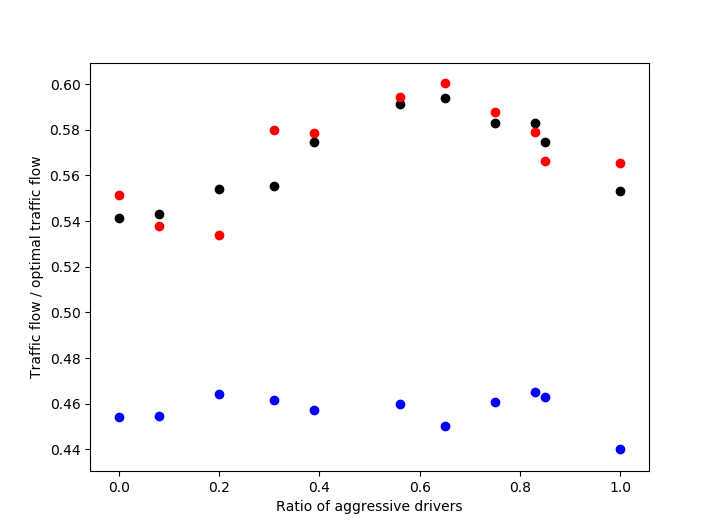
\includegraphics[scale=0.4]{figs/jam_flow_aggresives_150.png}
%    \caption{Traffic flow as a function of the ratio of agressive drivers versus passive drivers. We can tell there appears to be a ratio at which the traffic flow is optimal}
%    \label{fig:jam_flow}
%\end{figure}



\begin{figure}[ht]     
      \centering
       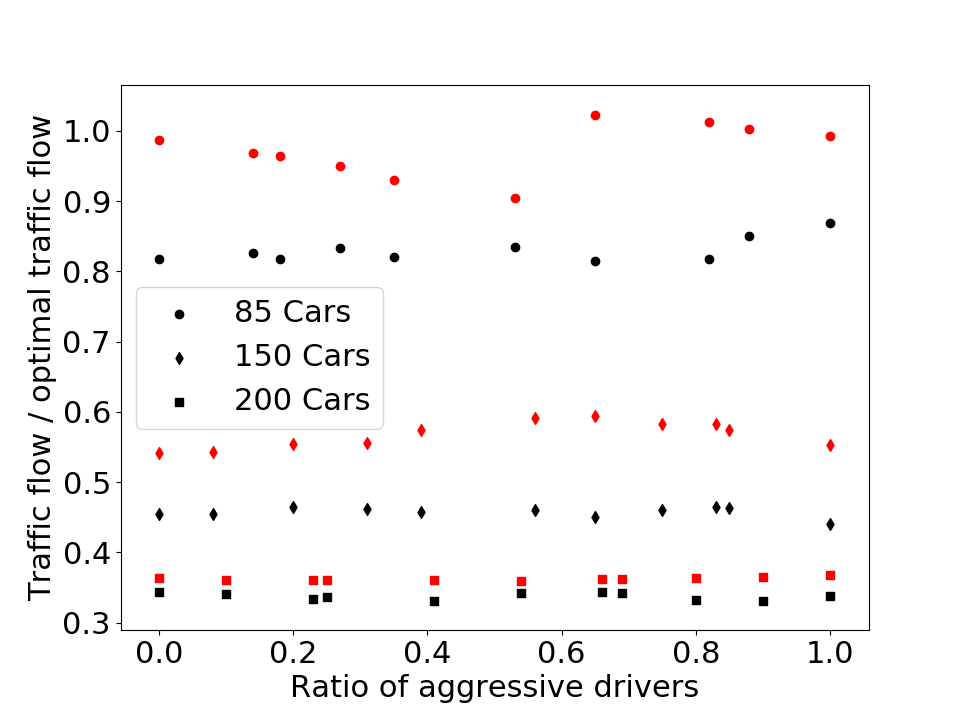
\includegraphics[scale=0.33]{figs/traffic_density_effect}
       \caption{Effect of artifical congestion on traffic flow for different values of traffic density and ratio of aggressive drivers. The red and black symbols are the average traffic flow before and after the introduction of an artificial disturbance, respectively. The measurements are done for three distinct traffic densities, representing low, medium and high density traffic. The traffic flow both before and after the disturbance decreases with increased density, with smaller shifts for higher densities. The effect of aggressive drivers is reduced  when traffic density is high. These measurments were done with $k_v=1.0$.}
       \label{fig:traffic_density}
 \end{figure}
 
\begin{figure*}[t]     
      \centering
       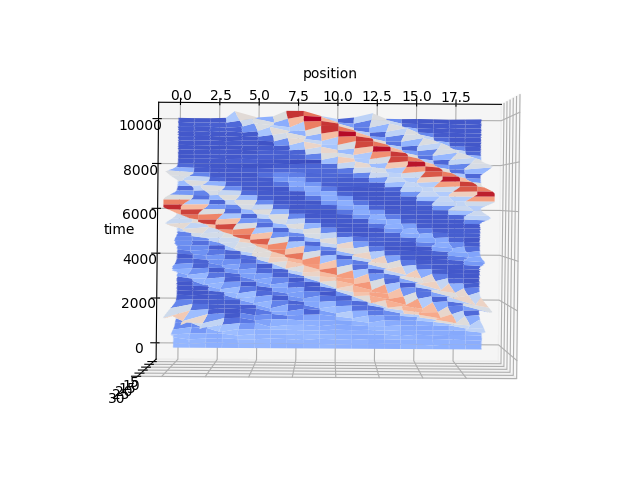
\includegraphics[scale=1, trim={1cm 2.5cm 1cm 3cm}]{figs/phase_transition1.png}
       \caption{Illustration of car density in the system going from an initial unstable, uniform distribution of cars to a state where congestions appear as waves. Regions with higher density are red, while low-density regions are blue. At time zero, the cars are uniformly distributed over the track separated in 20 buckets with periodic boundary conditions. As time progresses along the y-axis congestions start to form, seen in bucket position two around time step 1000. The cars are driving in positive bucket direction, but the congestions in seen moving in the reverse direction. The formed congestion wraps around and grows in density continously forming the red ridge moving from bucket position 20 to 0 from time step 2000 to 6000. Another feature is the small density ridge starting at bucket position 20 at time 4000 and then suddenly thinning out and disappearing at time 8000. This means the small congestion managed to resolve itself. }
       \label{fig:phase_transition}
 \end{figure*}

 
\begin{figure*}[t]
    \centering
      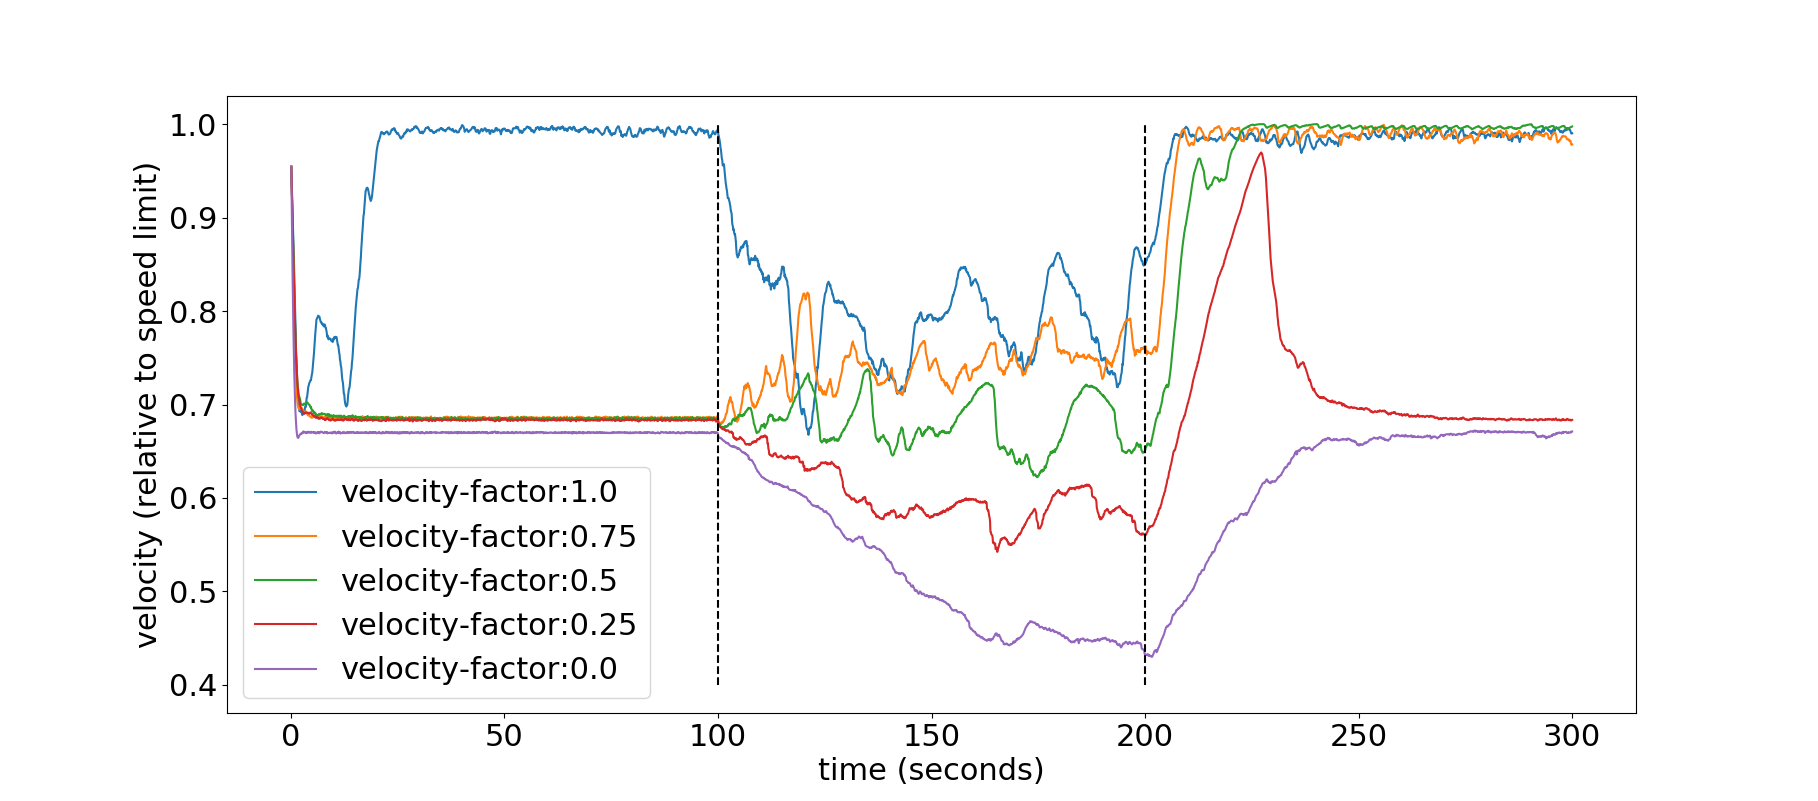
\includegraphics[scale=0.35, trim={0 0 0 0 }]{figs/velocity_over_time.png}
      \caption{Effect of varying velocity parameter on the average velocity in a system with an artifical disturbance introduced at time 100 and removed at time 200. In the first stage with uniform initialization all cars drive at the speed limit. All models drop almost immediately to around 0.7 and stay there. Only the model with velocity awareness of 1.0 is able to recover to the speed limit. During the disturbance, congestions form disrupting the steady-state. After the disturbance, the models with low velocity awareness decrease in average velocity whereas the models with higher velocity awareness actually increased their average velocity and managed to reach a higher velocity steady-state.}
      \label{fig:vel_over_time}
\end{figure*}
 
\begin{figure*}[t]     
      \centering
       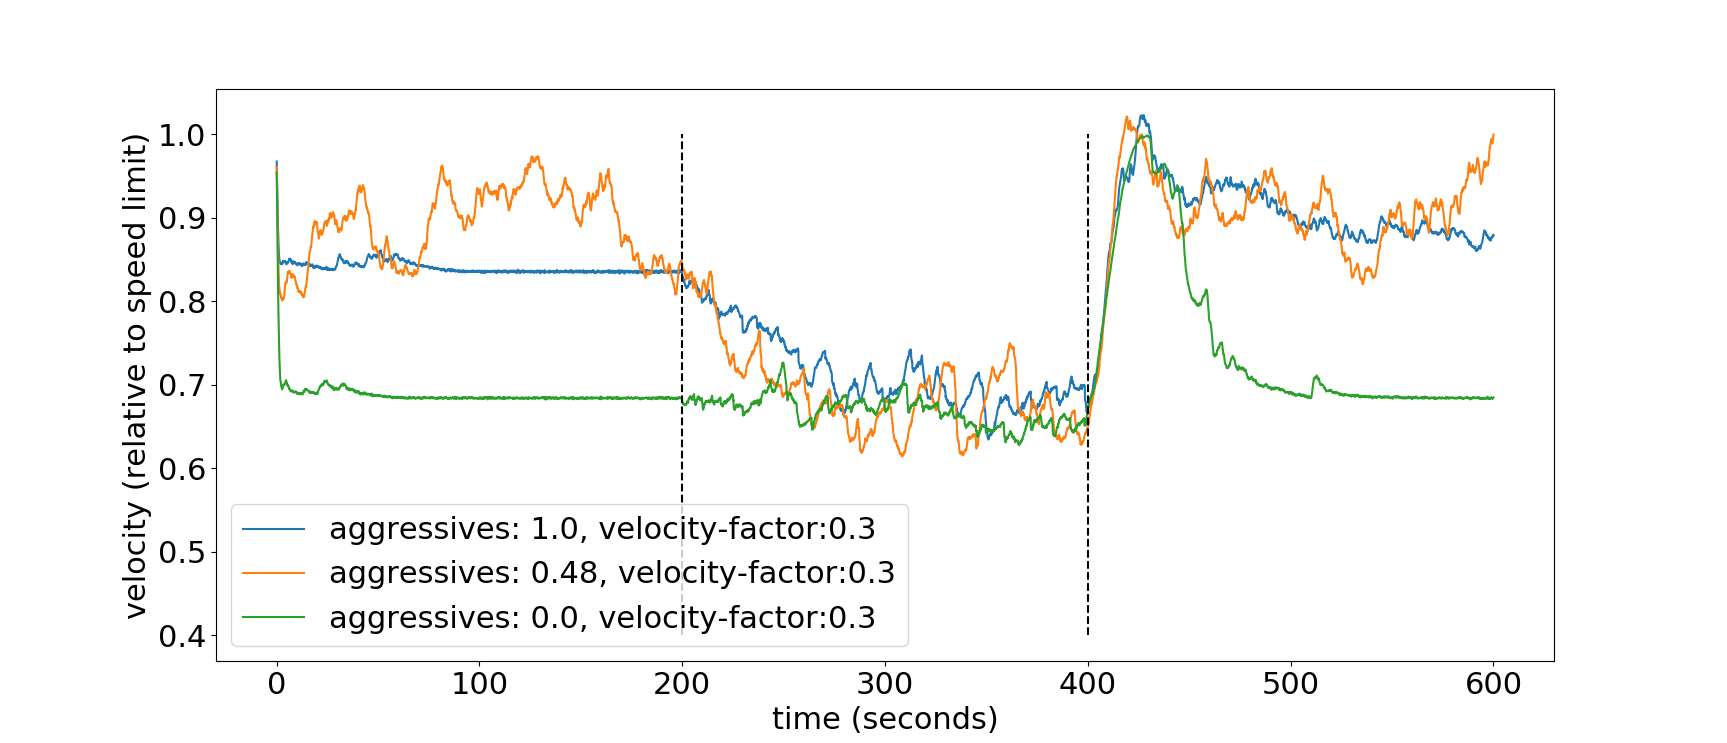
\includegraphics[scale=0.35]{figs/velocity_over_time_aggressive.png}
       \caption{Effect of mixed populations on the avergae velocity in a system with an artifical disturbance introduced at time 100 and removed at time 200. The system with a mixed population do not reach a steady state and have a high average velocity. All systems are equally affected by the disturbance. While the other two systems approach their steady state again when the disturbance is removed, the mixed system continues to oscillate close to the speed limit. }
       \label{fig:vel_agg_over_time}
 \end{figure*}

 \subsection{Congestion for varying density}
 One of the most important parameters for the formation and dissipation of traffic jams is known to be the traffic density \cite{kerner96trafficjam, kerner97flow}. We examined the effect of road saturation by varying the number of cars on a three-lane highway and measuring the average traffic flow  before and after an artificial disturbance had been introduced. The artificial disturbance was used to get an even, strong congestion for all cases and not rely on eventual self-formed congestions due to system instability.  We also varied the ratio of aggressive drivers in traffic to see if a more active lane-changing behaviour and shorter safety distances would have an effect on the traffic flow.
 
 The resulting measurements of traffic flow as a function of traffic density and ratio of aggressive cars is seen in figure \ref{fig:traffic_density}. The density measurements were done for three distinct values, 85, 150 and 200 cars representing low, high and medium densities, respectively. A system with fewer cars is sparse enough to not be affected by a blocked lane, cars have enough space to simply switch lanes and avoid the congestion, while a system with more than about 200 cars is so saturated that congestions form almost instantly.
 
 The measurements before the disturbance are the red symbols in the figure, while the measurements after are black. A clear difference in traffic flow before and after the congestion is observed for all car densities. However, the effect is more limited for higer densities. This could probably be explained by the fact that a highly saturated road forces drivers to slow down because of the decreased available distance between each car, placing the system in a congestion-like state from the beginning.

 The variations due to the ratio of aggressive drivers are seen along the x-axis in Figure \ref{fig:traffic_density}. The flow is close to constant, with small flucations, for all values. The exception is a slight rise in traffic flow for a large amount of aggressive cars in the case of low density traffic. The difference can by explained by the fact that the aggressive cars need available extra space to be able to have an effect. When the traffic is too dense, they get stuck at the same speed as the normal cars. Conversely, when there is available space, as in the case of low density traffic, the aggressive cars can take advantage of their higher speed and increase the over all flow of traffic.  

 The absence of change between individual measurements is possibly a consequence of the averaging used. The average is taken over a large time in the system both before and after the disturbance. Transient behaviour in the transition from flowing traffic to congestion is therefore averaged out and figure \ref{fig:traffic_density} only represents the steady-state behaviour. To study the transient behaviour of the system with the introduction of disturbances we examined the time evolution of the instantaneous velocity, see section \ref{sec:vel_param}. 

\subsection{Traffic congestion as a phase transition} \label{sec:phase}
Traffic congestions can be created by introducing obstacles or giving the cars a non-uniform initial distribution. Congestions can also appear without any such initial perturbation. This can be regarded as a phase transition in an unstable dynamical system \cite{bando1995dynamical}. When the velocity awareness in our model is high, the flow appears stable. Under a certain threshold of velocity awareness, congestions appear spontaneously as waves. This is illustrated in Figure \ref{fig:phase_transition}. At $t=0$ we see the cars evenly distributed. Between $t=0$ and $t=1000$ we see a how a wave starts forming, propagating backwards relative to the driving direction. We can observe a secondary smaller wave forming shortly after the primary wave, and a few more even smaller waves. Two of the small waves merge with the primary large wave, and one of them dissolves spontaneously at $t \approx 8000$. 

\begin{comment}
    Discussion here
\end{comment}

\subsection{Varying the velocity parameter}\label{sec:vel_param}
Figure \ref{fig:vel_over_time} displays the time evolution for varying velocity parameters \eqref{eq:velo_param}. The initial observation phase shows that the average velocities tend to drop to around 0.7.
This should correspond to the steady state where every car keeps their desired safety distance to the car in front.% see section REFERENCE TO SECTION and the theoretical value from equation REFERENCE EQUATION is X.
An interesting observation is that when the velocity awareness is set to 1.0, the model initially drops close to 0.7, but manages to recover to the speed limit. %DISCUSS THIS

Once a disturbance is introduced (first vertical line), the system leaves the steady state and starts fluctuating. For low velocity awareness values, the average velocity decreases, but for the larger velocity awareness the average velocity tends to increase.
After the disturbance is removed, the models with low velocity awareness slowly return to the steady state, whereas the other models manage to go all the way to the speed limit. This behaviour of escaping from a steady state to another, less stable steady state, can be likened to a system with a stable and unstable attractor (such as a simple pendulum). In and of itself, the system will always converge to the stable attractor, but external factors (in this case velocity awareness) can keep the system semi-stable in the unstable fix point.

This result is extremely interesting, since it implies that major traffic distrubances (such as a roadblack or accident) can actually improve the overall flow. Both during the disturbance and after it has been cleared up.
There have been studies that show that placing certain obstacles in front of an emergency exit improves the overall flow \cite{yanagisawa2009obstacle}, which lends some strength to this very unintuitive conclusion.

A likely reason that we don't commonly see this kind of flow improvement in the real world is that human drivers have a very low velocity awareness. With the advent of self driving cars however, it's possible that traffic disturbances  will no longer cause immense slowdowns, but might rather be beneficial (in small amounts).

\subsection{Effect of mixed populations on steady state}
In the previous section we studied the effect of velocity awareness and saw that a disturbance can have a positive impact on the flow. We have also previously studied mixed population of aggressive and normal drivers. Together, this raised the question whether a mix of driving styles can provide a continuous stream of micro disturbances and improve the overall flow. Figure \ref{fig:vel_agg_over_time} shows just that.
Populations with 100\% normal and 100\% aggressive drivers immediately go to their respective steady state and stay there until a disturbance. Since the aggressive drivers have a smaller safety distance (and higher speed limit), their steady state line is significantly higher. The mixed population never reaches a steady state and, most interestingly, it mostly stay above the purely aggressive population. This confirms our theory that mixed populations can help the system perform better than the sum of it's parts (which would correspond to the average between both steady states).

During the disturbance, the population with only normal cars starts oscillating but doesn't really decrease, whereas the other two populations drop to the same level. As soon as it clears up the mixed population shoots back up to the previous levels whereas the other two populations go up, but then start drifting down towards the steady states.

These results are very interesting. Intuition tells us that a population of aggressive drivers should have the highest velocity since every car wants to drive faster and keep a smaller distance to the car in front. The simulations however, show that a mixed population adds some randomness to the system which can be beneficial for breaking up congestion and steady state behaviour.

\section{Conclusion}
The model succesfully predicts the formation of congestions with a clear dependence on traffic density. A system with low traffic density has a higher steady-state flow, but is relatively more affected by an artifical disturbance creating congestion due to the initial higer average flow. Propagating congestion waves due to stop-and-go behaviour are shown to form spontaneously in systems with high traffic density. 

Driver behaviour, in terms of aggressiveness and neighbour-velocity adaptation, has an effect on both steady-state flow and transient behaviour in transitions between steady-state and congestions. The velocity adaptation decreases the rate at which congestions form and allows for higher traffic densities in steady-state flow. For the transient behaviour, both a higher ratio of aggressive drivers and a higher degree of velocity adaptation decreases the effect of an artificial disturbance and give the system a higher rate of recovery to a state with optimal traffic flow.

The model used is relatively simple and represents an idealized view of driver behaviour and the physical properties of highway traffic. Even though the results are qualitatively pointing towards a positive effect of the introduction of velocity adaptation capabilities, the results should probably not be seen as more than an pointer in the right direction. To achieve conclusive results further study is needed to improve the model as well as to perform a more extensive search in parameter space. An initial main direction for further work would be to investigate more complex additions, such as driver reaction time, noise in velocity measurements, decreased vision when changing lanes et cetera.

%\section{Parameter dependence of cluster formations etc...}

%\subsection{}

% Figurer inkluderade som eps-filer
%% \begin{figure}\centering
%% \includegraphics{filnamn.eps}
%% \caption{\label{figuren} Perioden $T$ som funktion av pendellängden.}
%% \end{figure}

% Figurer inkluderade med xfigs postscript+latex
%% \begin{figure}\centering
%% \input{filnamn.pstex_t}
%% \caption{\label{finafiguren} Perioden $T$ som funktion av
%%   pendellängden.}
%% \end{figure}
\bibliographystyle{unsrt}
\bibliography{bibliography}

\end{document}
